% \documentclass[a4paper, technote, compsoc]{IEEEtran}
\documentclass[../../thesis.tex]{subfiles}

\newcommand{\inner}[2]{\left<#1, #2\right>}
\newcommand{\alemap}{\ensuremath{\mathcal{A}}}
\newcommand{\dt}{\ensuremath{\Delta t}}
\newcommand{\pexp}{\ensuremath{\frac{2\gamma}{\left(\gamma-1\right)}}}
\newcommand{\aleX}{\ensuremath{\mathcal{X}}}
\newcommand{\Ah}[1]{\ensuremath{\vb{#1}^{n+1}_h}}
\newcommand{\Ahn}[1]{\ensuremath{\vb{#1}^{n}_h}}

\newcommand{\rbV}{\ensuremath{\mathbb{V}}}
\newcommand{\rbVT}{\ensuremath{\rbV^T}}
\newcommand{\epspod}{\ensuremath{\varepsilon_\text{POD}}}

\begin{document}

\section{Results and Certification}
We are now going to see the Hyperreduced Order Model in action.
The error decay for the solution and the nonlinear operator 
are presented and commented in Section~\ref{sec:hrom_results_reduced_basis}.
% we will study the interaction between the approximation errors
% from the RB and the nonlinear operator bases.

Finally, in Section~\ref{sec:hrom_results_posteriori_error_estimation} we show 
how to certify the HROM solution with a model truncation technique.  

\subsection{Approximation Error}
\label{sec:hrom_results_reduced_basis}
We explore how the number of modes influences the approximation error of the FOM solution.

Since we are using a POD to build our reduced basis, 
we attempt to relate the POD a posteriori error estimations with 
the actual error between ROM and FOM.

\subsubsection{POD: A Posteriori Errors}
The POD returns a collection of vectors and sigular values, each related to the other.
The magnitude of each singular value somehow encodes 
how much information is carried by its associated vector about the original span.
% Departing from the idea that we need at least \textit{one} basis element to solve our problem,
% and that we have a finite amount of 

We define the energy of the basis that contains up to the $i$-th element as
\begin{equation}
    \mathcal{E}_i = \frac{\sum_{j=0}^{i}\sigma_j^2}{\sum \sigma_k^2}.
\end{equation}
We shall see if this variable has any predictive power on the ROM error.

\subsubsection{ROM Optimal Size}
We want to find the smallest size $N^{*}$ for which the FOM is correctly reproduced.
Naturally, the exact value of this variable is problem-dependent, 
but the way in which we approach its search would suit any RB problem.

In Figure~\ref{fig:error_decay} we present the ROM error with respect to the number of basis elements and the energy of the truncated basis.
\begin{figure}[h]
    \centering
    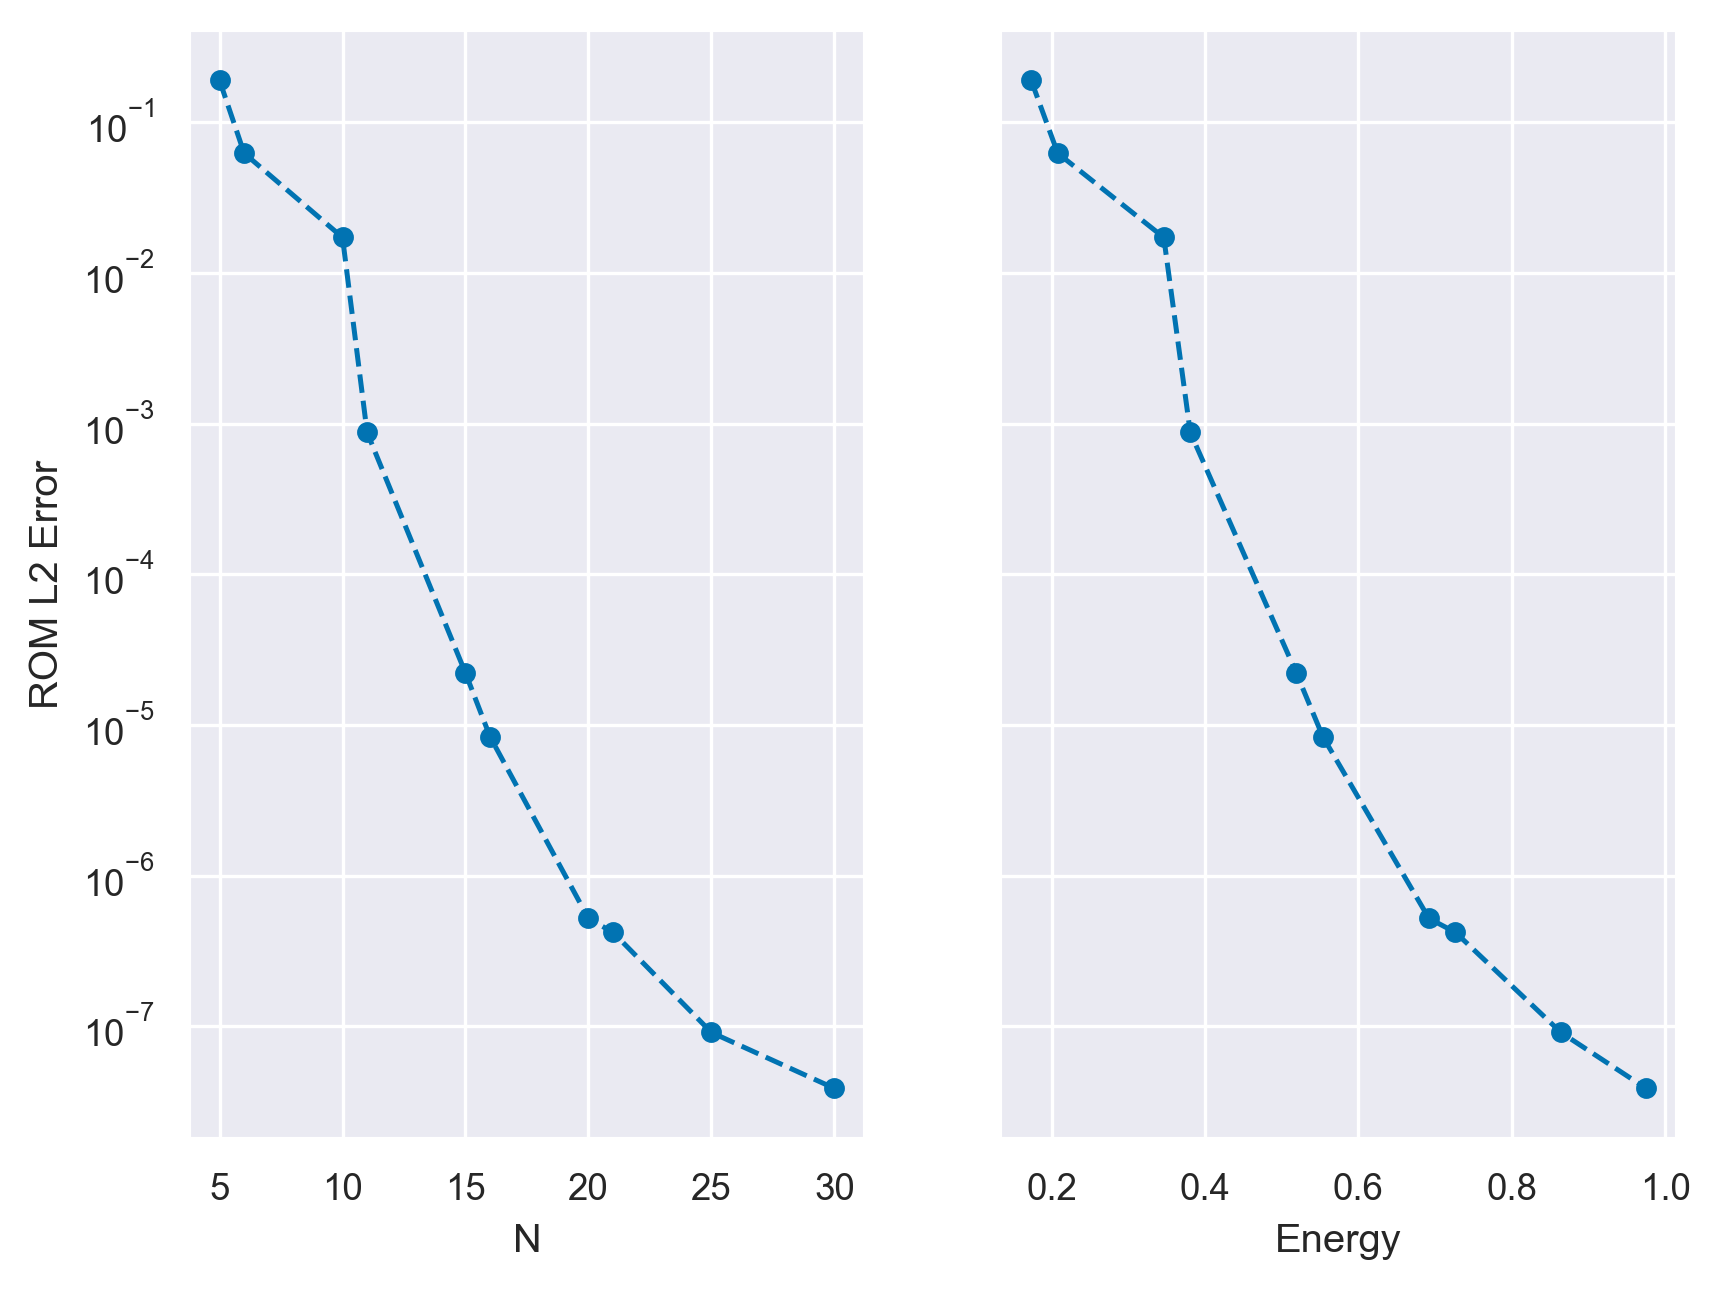
\includegraphics[width=\columnwidth]{research_project/piston/figures/rb_certification/error_decay.png}
    \caption{Error decay for number of basis elements and basis energy level.
    Expectedly, the more basis elements we have, the lower the error.}
    \label{fig:error_decay}
\end{figure}
The more elements in the basis, the smaller the error.
The more energy the basis contains, the better the approximation.

We present in Figures~\ref{fig:outflow_model_comparison_N_5} and \ref{fig:outflow_model_comparison_N_10} 
the actual solution at the outflow for each model (FOM and ROM).
We can see how the ROM model is poorly resolved for $N=5$, as reflected by the error,
but how it drastically improves for $N=10$, except for the initial instants of movement.
\begin{figure}[h]
    \centering
    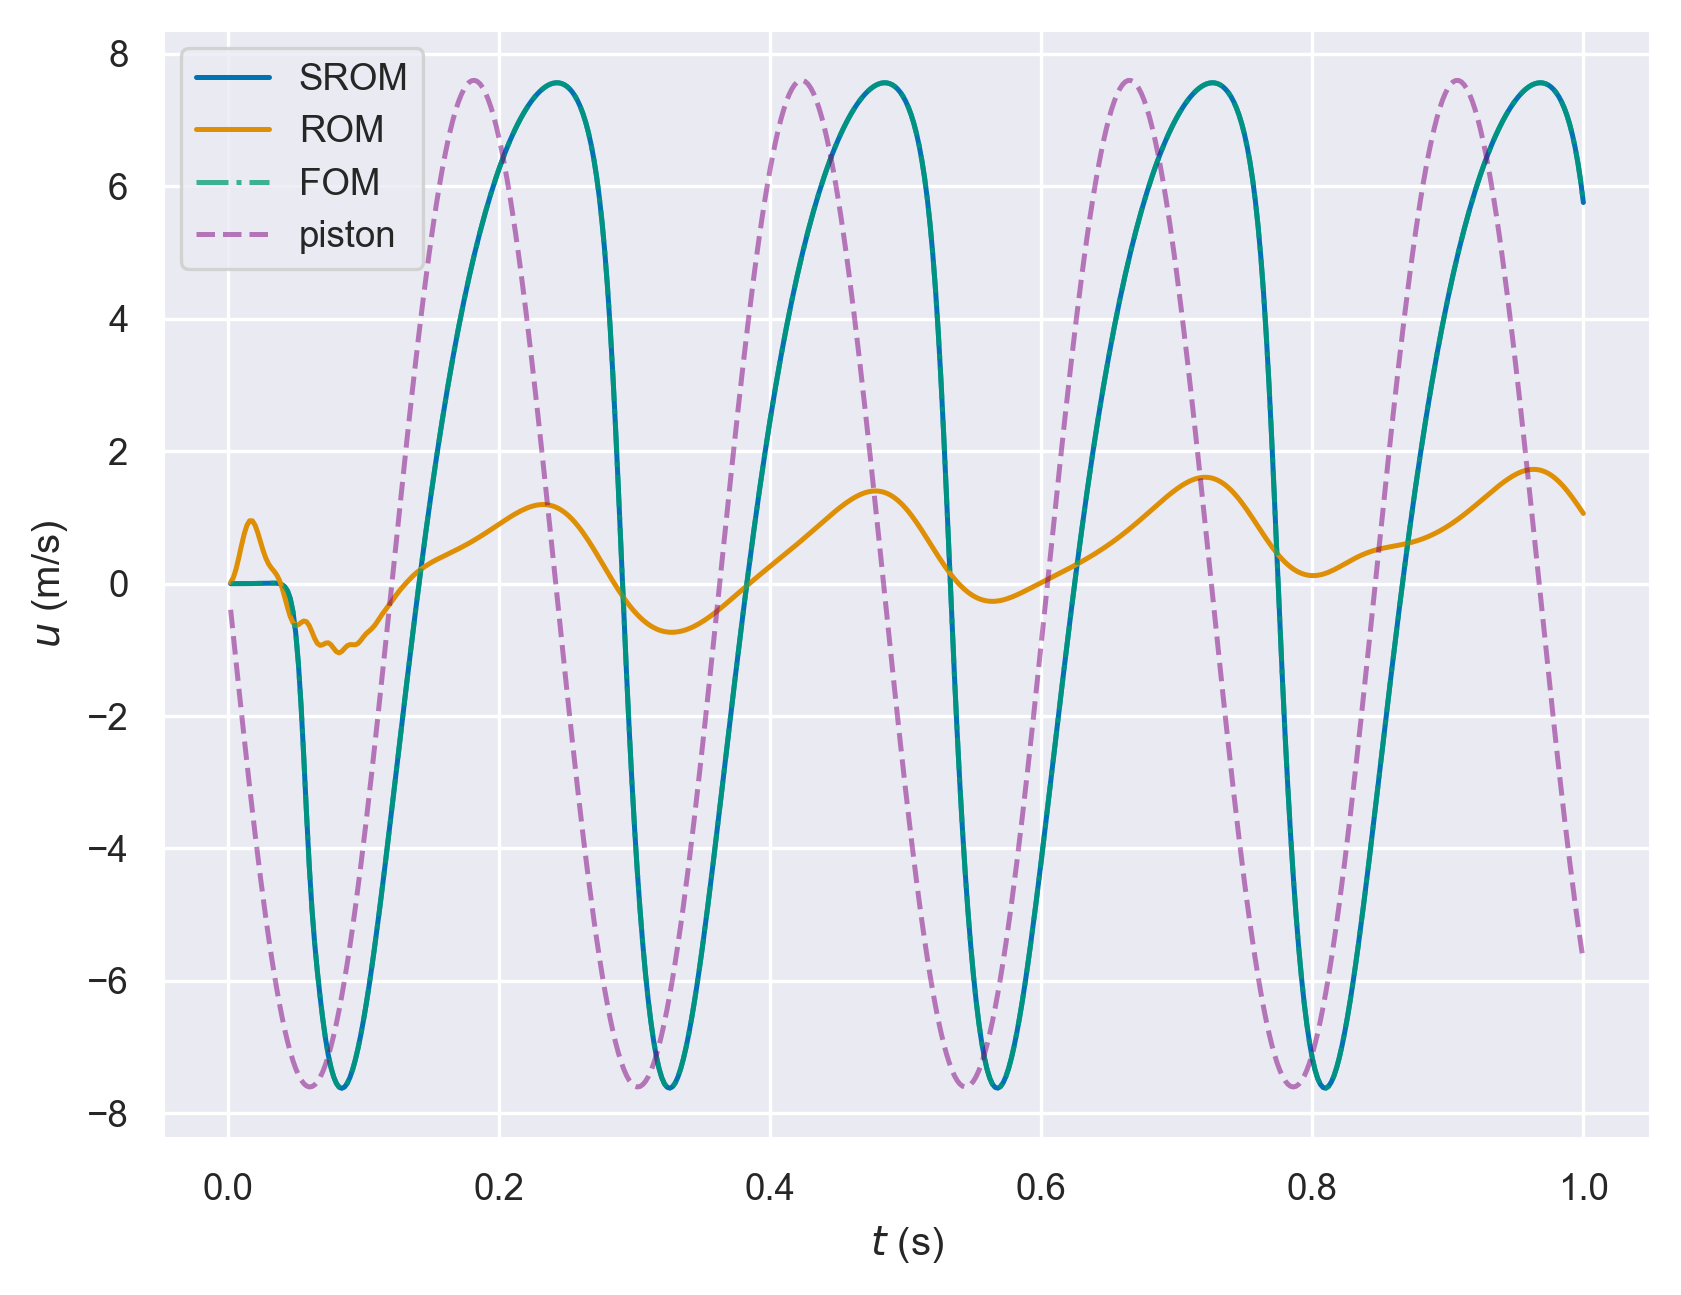
\includegraphics[width=\columnwidth]{research_project/piston/figures/rb_certification/outflow_probes_comparison_rom_5_srom_15_online_0.png}
    \caption{Outflow velocities for different models. The ROM model is poorly resolved for $N=5$.}
    \label{fig:outflow_model_comparison_N_5}
\end{figure}
\begin{figure}[h]
    \centering
    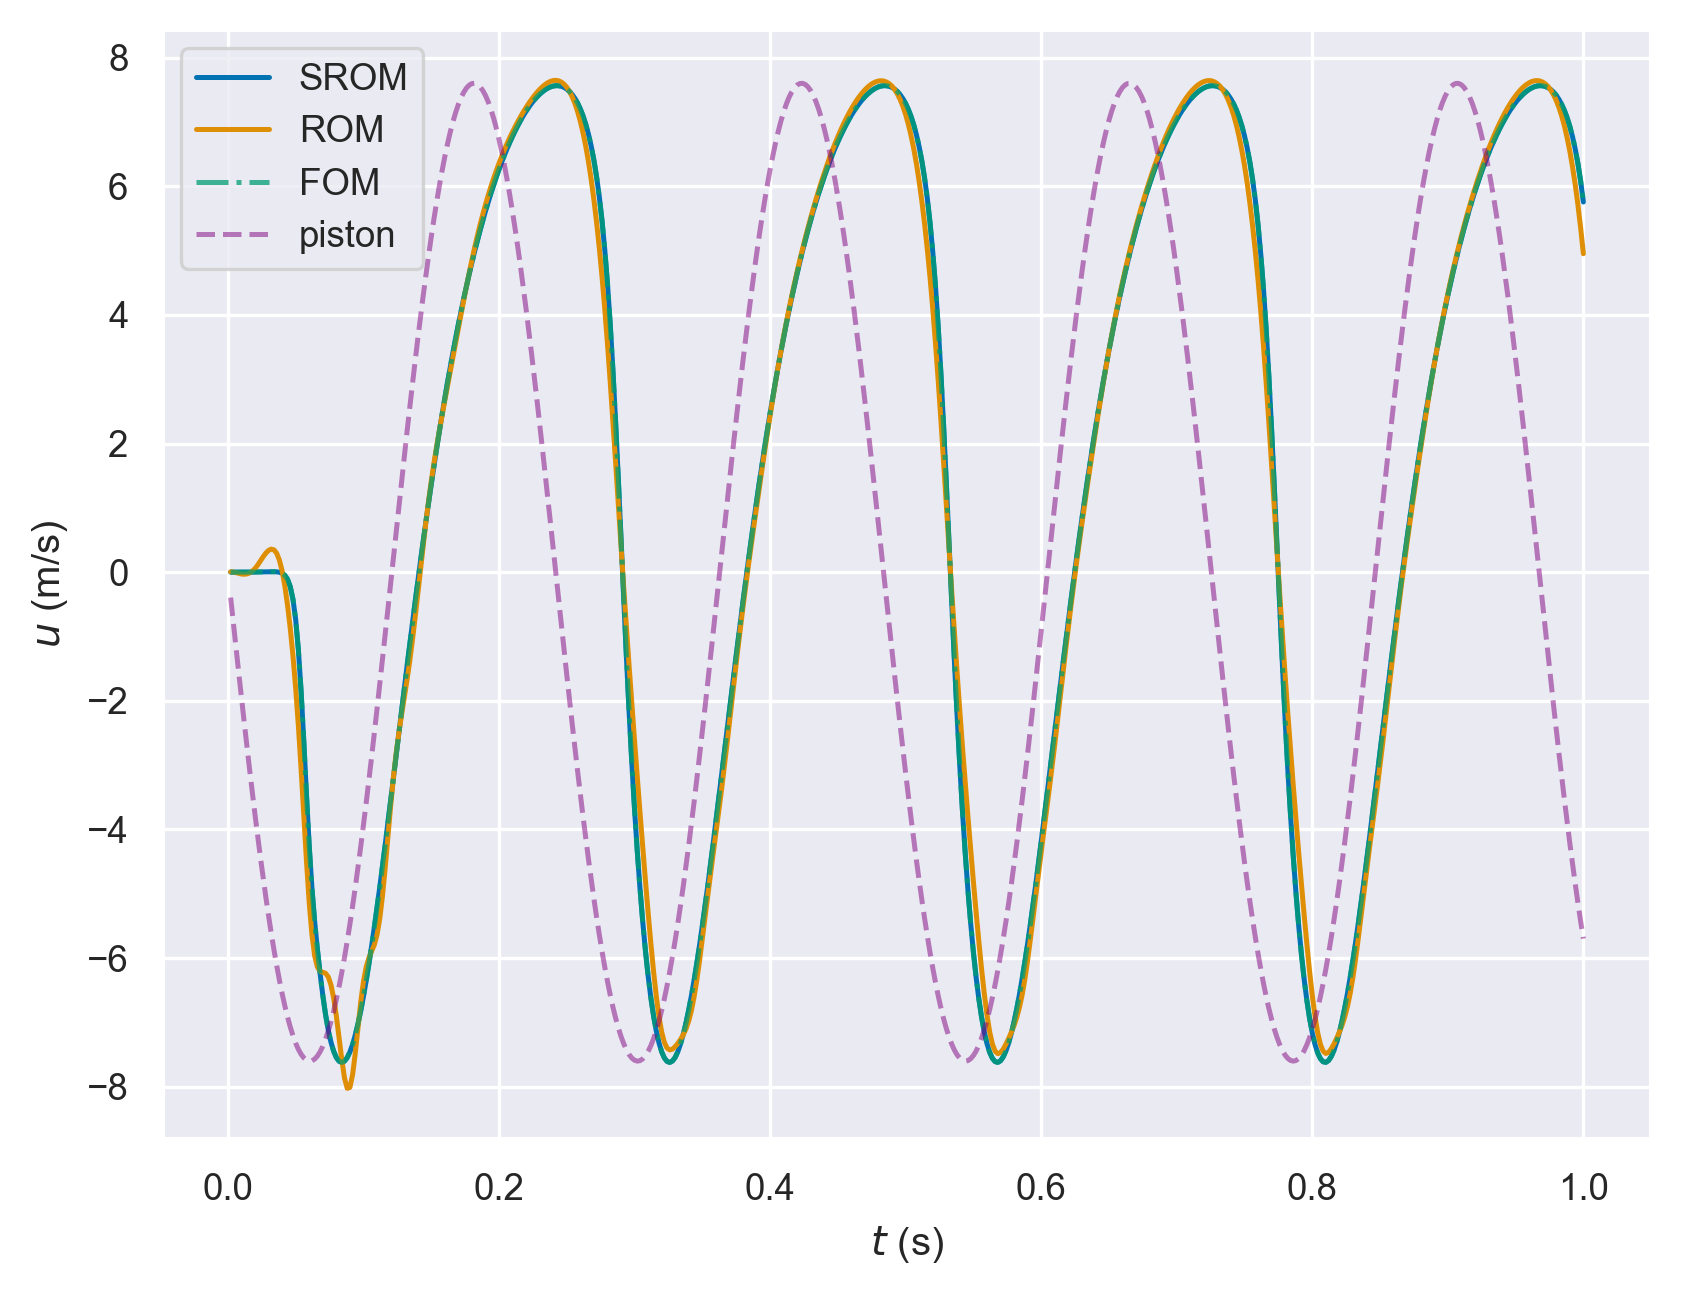
\includegraphics[width=\columnwidth]{research_project/piston/figures/rb_certification/outflow_probes_comparison_rom_10_srom_20_online_0.png}
    \caption{Outflow velocities for different models. 
    The ROM model is better resolved for $N=10$, except at the beginning of the simualation.}
    \label{fig:outflow_model_comparison_N_10}
\end{figure}
\mytodo{Use enhanced POD technique to solve this problem.}
The flow departs from rest as the piston starts to move.
Therefore, the first snapshots contain a nonlinearity in the sense that the flow starts to move on one side, 
but remains still along the rest of the tube.

However, for most of the time interval, this kind of nonlinearity will not be present again,
since the flow will be in constant motion, flowing in and out of the system.
Hence, it is an expected behaviour that this is the interval where the ROM will fail the most,
unless we include a sufficient number of basis elements.
To fix this problem, certain techniques exist which enhance the basis without adding excessive complexity.

\subsection{(M)DEIM Error Estimation}
TBD.

\subsection{HROM Error Estimation}
\label{sec:hrom_results_posteriori_error_estimation}
To compute the HROM error in the preceding sections
we required the assembly and solution of the FOM model.
This is an undesirable fact, since if to validate our ROM solution
we need to compute its FOM counterpart, 
we are better off computing straightaway the FOM model 
(which will be absolutely accurate).

Hence, we need an efficient a posteriori error estimator.

\subsubsection{Sacrificial ROM}
We use the \textit{model truncation} technique.
That is, we are going to carry with us \textit{two} ROMs,
with different basis elements.

The second one, called \textit{sacrificial} ROM (SROM),
will be used to compute the actual error for the base ROM,
without requiring the calculation of the FOM.
\mytodo{Create descriptive flow chart.}
The SROM is baptized with such name because its results cannot be used,
since we have no way to estimate their error.
We assume it is smaller than the one of base ROM, since it has more basis elements,
but we cannot know how much smaller it is.
Hence, it is an additional ROM whose results we use to estimate the error of the former, 
and nothing else.

For this error estimation procedure, the question we seek answering is:
\textit{how many more nodes needs the SROM to carry to certify with accuracy the base ROM?}
Again, the answer to this question is problem-dependent,
but our approach to find it could be used for any other problem.

\subsubsection{Error Estimation}
We depart from the error we seek to bound,
and proceed to add and susbtract the solution from the sacrificial ROM,
\begin{equation}
    \norm{u_h - \rbV_{N} u_N} = \norm{u_h \pm \rbV_{\hat{N}} u_{\hat{N}} - \rbV_{N} u_{N}},
\end{equation}
where $\hat{N} > N$. 
By the triangle inequality, we get
\begin{equation}
    \norm{u_h - \rbV_{N} u_N} \leq \norm{u_h - \rbV_{\hat{N}} u_{\hat{N}}} + \norm{\rbV_{\hat{N}} u_{\hat{N}} - \rbV_{N} u_{N}}.
\end{equation}
If we define the error function $e_N = \norm{u_h - \rbV_{N} u_N}$, 
we get an upper bound of the desired error in terms of the sacrificial ROM error and the error between ROMs,
\begin{equation}
    e_N \leq e_{\hat{N}} + \norm{\rbV_{\hat{N}} u_{\hat{N}} - \rbV_{N} u_{N}}.
\end{equation}
With sufficient RB elements, it should be safe to assert that the error made 
with additional modes should be smaller or equal to the one made without it,
\begin{equation}
    e_{\hat{N}} \leq e_{N}.
\end{equation}
Thus, we get the following error bound,
\begin{equation}
    e_N \leq \norm{\rbV_{\hat{N}} u_{\hat{N}} - \rbV_{N} u_{N}},
\end{equation}
It remains to determine how sharp this error estimate is.

\subsubsection{Error Between Two ROMs}
The error estimator 
\begin{equation}
    \tilde{e}_{N}(\hat{N}) = \norm{\rbV_{\hat{N}} u_{\hat{N}} - \rbV_{N} u_{N}},
\end{equation}
can be expressed as a sum in terms of the RB elements.
Due to the hierarchical character of the RB basis, $\rbV_{\hat{N}}$ contains the same elements 
up to $N$ as $\rbV_{N}$.
Thus, the error between ROMs can be expressed like
\begin{equation}
    \begin{split}
        \norm{\rbV_{\hat{N}} u_{\hat{N}} - \rbV_{N} u_{N}} 
        = \\ 
        \norm{
        \sum_{i=N+1}^{\hat{N}} u^{\hat{N}}_{i} \psi_{i} 
        + 
        \sum_{j}^{N} (u^{\hat{N}}_{j} - u^{N}_{j}) \psi_j
        }.
    \end{split}
\end{equation}
The difference $(u^{\hat{N}}_{j} - u^{N}_{j})$ between ROM coefficients should be relatively small, 
since it represents the difference between the two coefficients associated to the same mode.
If they were notably different, 
it would mean that the dynamics between the original ROM and the sacrificial one are different.
Since the basis is hierarchical, this effect is unlikely to happen: 
adding an additional mode should only refine the solution, 
not change drastically how the previous modes are scaled.
They are not strictly the same because the ROM matrix changes if more modes are added to the basis,
but again, it does so in a way that dynamics should be preserved.

In Figure~\ref{fig:estimator_accuracy} we present how close is the estimator to the actual error.
We have computed the estimator for~\mbox{$\Delta N = 1, 5$} and~$10$ additional modes.
Then, we compute \textit{estimator accuracy}, how far it is from the actual ROM error,
aggregated for all timesteps, 
\begin{equation}
    \text{Estimator Accuracy} = \norm{e_t - \tilde{e}_t} 
\end{equation}
\begin{figure}[h]
    \centering
    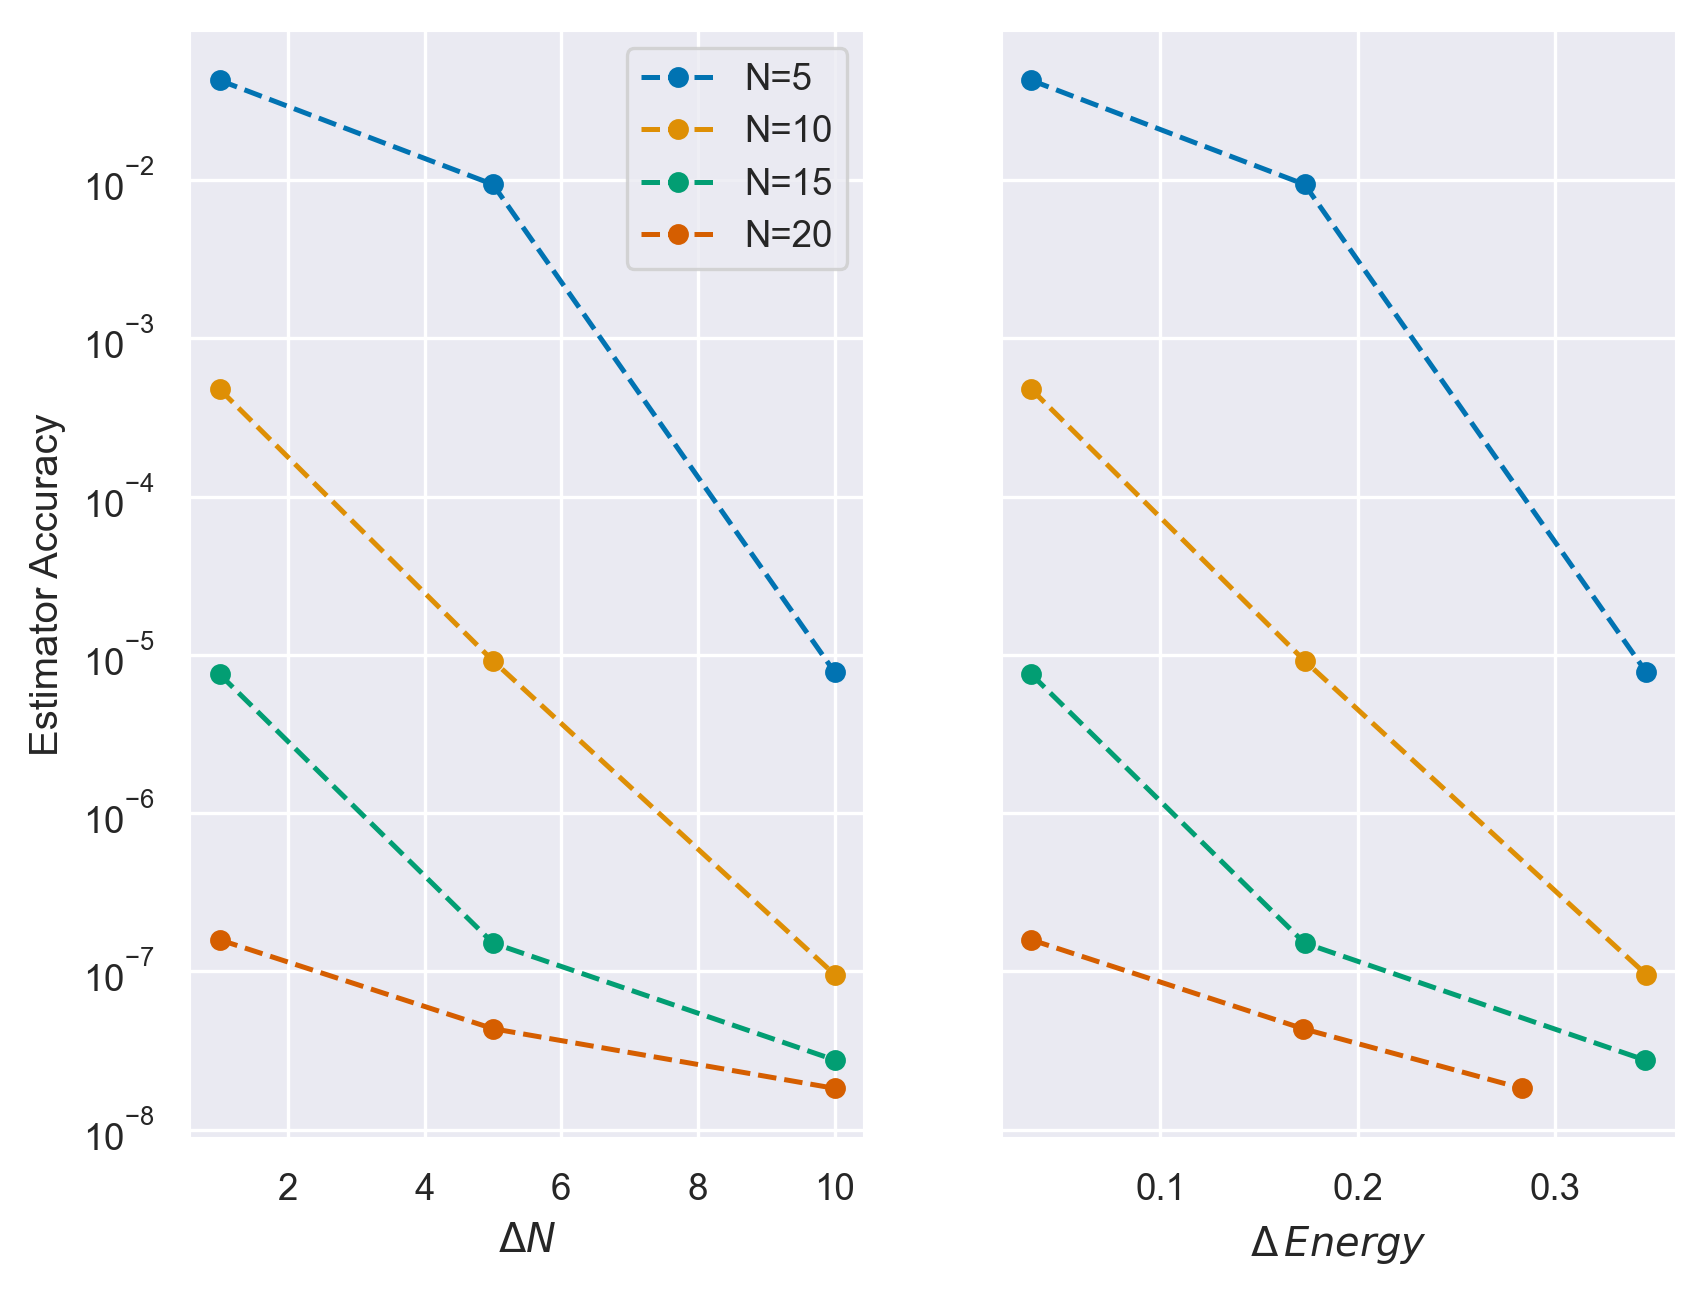
\includegraphics[width=1\columnwidth]{research_project/piston/figures/rb_certification/estimator_accuracy.png}
    \caption{A posteriori error estimator accuracy.
    We see how it can become more effective to carry more additional modes than rather just one.}
    \label{fig:estimator_accuracy}
\end{figure}
We conclude that it seems to be better to carry more than one mode.
Nevertheless, if it is going to become too costly to compute all these additional modes,
one extra mode could do the job fairly well too, provided that the base ROM is well resolved.

\subsubsection{RB and MDEIM Error Interaction}
TBD. 

\end{document}